%  article.tex (Version 3.3, released 19 January 2008)
%  Article to demonstrate format for SPIE Proceedings
%  Special instructions are included in this file after the
%  symbol %>>>>
%  Numerous commands are commented out, but included to show how
%  to effect various options, e.g., to print page numbers, etc.
%  This LaTeX source file is composed for LaTeX2e.

%  The following commands have been added in the SPIE class 
%  file (spie.cls) and will not be understood in other classes:
%  \supit{}, \authorinfo{}, \skiplinehalf, \keywords{}
%  The bibliography style file is called spiebib.bst, 
%  which replaces the standard style unstr.bst.  

\documentclass[]{spie}  %>>> use for US letter paper
%%\documentclass[a4paper]{spie}  %>>> use this instead for A4 paper
%%\documentclass[nocompress]{spie}  %>>> to avoid compression of citations
%% \addtolength{\voffset}{9mm}   %>>> moves text field down
%% \renewcommand{\baselinestretch}{1.65}   %>>> 1.65 for double spacing, 1.25 for 1.5 spacing 
%  The following command loads a graphics package to include images 
%  in the document. It may be necessary to specify a DVI driver option,
%  e.g., [dvips], but that may be inappropriate for some LaTeX 
%  installations. 
\usepackage[]{graphicx}
\usepackage{caption} 
\usepackage{subcaption} 
\usepackage{hyperref}
%\usepackage{mathtools}

\title{CT Thermometry with Image Registration and Filtering} 

%>>>> The author is responsible for formatting the 
%  author list and their institutions.  Use  \skiplinehalf 
%  to separate author list from addresses and between each address.
%  The correspondence between each author and his/her address
%  can be indicated with a superscript in italics, 
%  which is easily obtained with \supit{}.

\author{Zachary DeStefano\supit{a}, Jack Yao\supit{a}, Nadine Abi-Jaoudeh\supit{a}, Ming Li\supit{a}
\skiplinehalf
\supit{a}National Institutes of Health, Clinical Center\\Bethesda, MD 20814
}

%>>>> Further information about the authors, other than their 
%  institution and addresses, should be included as a footnote, 
%  which is facilitated by the \authorinfo{} command.

\authorinfo{Author Emails: zdestefa@uci.edu}
%%>>>> when using amstex, you need to use @@ instead of @
 

%%%%%%%%%%%%%%%%%%%%%%%%%%%%%%%%%%%%%%%%%%%%%%%%%%%%%%%%%%%%% 
%>>>> uncomment following for page numbers
% \pagestyle{plain}    
%>>>> uncomment following to start page numbering at 301 
%\setcounter{page}{301} 
 
  \begin{document} 
  \maketitle 

%%%%%%%%%%%%%%%%%%%%%%%%%%%%%%%%%%%%%%%%%%%%%%%%%%%%%%%%%%%%% 
\begin{abstract}
Monitoring temperature during a cone-beam CT (CBCT) guided ablation procedure is important for prevention of over-treatment and under-treatment. In order to accomplish ideal temperature monitoring, a thermometry map must be generated.  Previously, this was attempted using CBCT scans of a pig shoulder undergoing ablation \cite{Li13}. We are extending this work by using CBCT scans of real patients and incorporating more processing steps. We register the scans before comparing them due to the movement of organs. We also employ a robust change metric due to image noise and artifacts. In order to achieve an automated system in the future, we use PCA to select the Region of Interest (ROI) where the needle tip is located and thus where the ablation occurred. Once we have generated a change map in the ROI, we correlate change data with temperature data at points in the region to transform our change map into a thermal map. This thermal map is then able to provide an estimate as to the size of the ablation zone. We repeated our procedure on a data set of 12 patients who had a total of 24 ablation procedures performed. We were able to generate reasonable thermal maps with varying degrees of accuracy. In addition to providing estimates of the size of the ablation zone, these maps were used to produce 3D visualizations of the ablation zone and needle.  
\end{abstract}

%>>>> Include a list of keywords after the abstract 

\keywords{Cone-beam CT, CBCT, Thermometry, Radiofrequency Ablation, Time Delay Analysis}

\section{Introduction}
\label{sec:intro}  % \label{} allows reference to this section

The possibility of generating a thermal map from CBCT scans has been explored before \cite{Li13}. We decided to extend the work to real patients and incorporate more processing steps to enhance the maps. For the procedures analyzed in this work, there was a baseline CBCT scan taken after the ablation needle was inserted but before it was heated. There were then 1-4 scans taken as the needle was heated and cooled.

These scans were taken a few minutes apart on live patients, thus there was movement of the organs. In order to account for this, we kept the baseline scan static and registered the subsequent scans to the baseline scan. This allowed us to have 3D CBCT scans that were reasonably aligned. However there was still noise, needle artifacts, and small registration errors. We thus needed a change metric that was robust to these issues. 

Computing the pixel by pixel difference between scans is a poor metric that is not robust enough for our needs. Using the Wronskian Change Detector was explored previously \cite{Li13} but it is not well suited for the regression calculation we need to perform. Using the values in a window around a pixel proved to be effective though. 

We compared windows around a pixel in the baseline scan and comparison scan using two different methods: Mean Difference and Spatial Offset RMSE. The mean difference method is equivalent to performing a convolution using an averaging filter on both images and then computing the difference image. The Spatial Offset RMSE method is equivalent to finding the ideal spatial offset between the windows and then computing the RMSE of the pixel values in the shifted signal. 

Because the relationship between HU change and temperature change varies depending on which organ is being affected \cite{Fani14}, it makes sense to only compute the thermal map for the ROI where the ablation occurred. Because the needle has distinct HU values from tissue and the ablation occurred at the tip of the needle, we were able to automate the process of finding the ROI. 

The Spatial Offset RMSE method is more computationally intensive than the Mean Difference method but it produces a much smoother change map. We thus use the Mean Difference to give us an estimate of the thermal map in order to verify that our ROI contains the ablation. We then use the Spatial Offset RMSE to compute a more accurate thermal map. 

\section{Related Work}

\subsection{CT Thermometry}

CT Thermometry has been explored since the late 1970's with some success \cite{Fani14}. Using linear regression, various attempts have shown relationships between HU unit value and temperature. Due to the varying thermal properties of different tissues, the exact calibration curve varies depending on which organ is being affected. It thus makes sense for us to only focus on the ROI around the ablation needle when generating a thermal map. 

Many of the attempts focused on correlating individual HU unit values with temperature. These values can be heavily influenced by image noise and metal artifacts. We thus decided to use a more robust change metric when correlating our HU unit change values with temperature change.  

\subsection{Image Registration}

Medical Image Registration has been researched extensively \cite{Oliveira14, Hill01}. For our purposes, we needed to align temporal sequences of CBCT scans. In particular, we performed an affine registration in order to account for movement of the organs during the ablation procedure. The organs can deform thus we also incorporated non-rigid registration. There is now an open source tool known as \href{http://cmictig.cs.ucl.ac.uk/wiki/index.php/NiftyReg}{NiftyReg} \cite{Ourselin01,Modat10} that was able to perform both the affine \cite{Ourselin01} and deformable \cite{Modat10} registration.   

\subsection{Wronskian Change Metric}

Previously, the Wronskian Change Detector \cite{Durucan01} was proposed as a metric that would be robust to noise \cite{Li13}. This particular change detector has been shown to perform well for classification problems \cite{Panda13,Durucan01,Ang11,Subudhi13} in image analysis. The formula however computes the ratios between intensity values. Because the relationship between HU unit value and temperature is roughly linear \cite{Fani14}, we need a function that increases linearly as the change in HU unit increases. Because the Wronskian function does not, we decided not to use it for our purposes. 

\subsection{Time Delay Analysis}

It is a common problem in signal processing to have two nearly identical signals that are offset by a delay. In order to calculate the most likely delay, cross-correlations are used \cite{Rhudy09}. The cross-correlation of two real-valued discrete signals $f$ and $g$ is defined as follows:
\[
(f \star g)[n] = \sum_{m=-\infty}^{\infty}{f[m]g[m+n]}
\]
The most likely delay $t_{delay}$ occurs when the correlation is the highest thus
\[
t_{delay} = arg\,max_t (f \star g)[t]
\]

For our purposes, we will take two square small images $U$ and $V$ and interpret them as periodic 2D signals that continuously repeat horizontally and vertically. Extrapolating from time delay analysis, the ideal spatial offset between the images occurs when the correlation is highest. Thus our ideal offset $(r,c)$ is as follows:
\[
(r,c)_{offset} = arg\,max_{r,c} \sum_{l=0}^{n-1} \sum_{k=0}^{n-1} {U_{k+r,l+c} \cdot V_{k,l}}
\]
Our change metric calculates the RMSE of the two images with this offset incorporated.


\section{Pipeline}

For each ablation procedure, there was a baseline CBCT scan as well as 1-4 comparison CBCT scans. The comparison scans were taken at various stages of heating and cooling the needle. For each comparison scan, a corresponding thermal map was generated via the following procedure:
\begin{enumerate}
\item Register the comparison scan to the baseline scan
\item Use Connected Component Analysis and PCA to detect the Needle tips
\item Use the result to find the ROI regions
\item Take the ROI regions found, filter the images, and calculate the difference
\item Use the result to find the ROI regions where the ablation likely occurred
\item Calculate the Spatial Offset RMSE value for the ROI regions found
\item Correlate Spatial Offset RMSE values from in the temperature zones with the temperature data
\item Use the regression model from the correlation calculated to generate a thermal map for the entire ROI
\end{enumerate}


\subsection{Image Registration}

For the registration step, the 3D comparison scan was registered to the 3D baseline scan using the software package NiftyReg. We used the \textbf{\href{http://cmictig.cs.ucl.ac.uk/wiki/index.php/Reg_aladin}{reg aladin}} command to perform an affine registration\cite{Ourselin01}. This was used to try to account for movement of the organs between different scans. We then used the \textbf{\href{http://cmictig.cs.ucl.ac.uk/wiki/index.php/Reg_f3d}{reg f3d}} command to perform non-rigid registration\cite{Modat10}. This was an attempt to align the organs in such a way that accounted for changes in their shape between scans. Figure \ref{beforeAndAfterReg} shows an example of image slices before and after registration. 

\begin{figure} 
\centering 
\begin{subfigure}[t]{0.45\textwidth} 
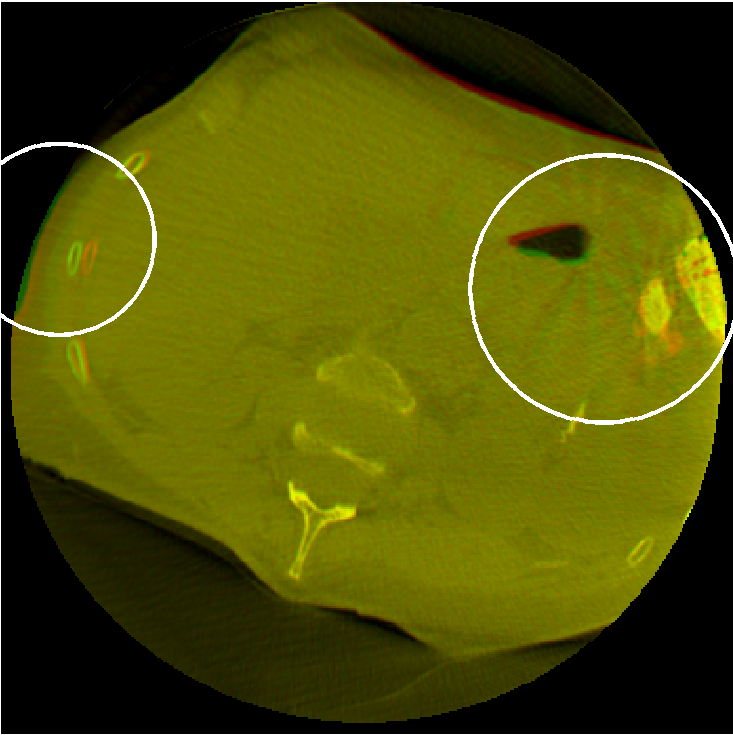
\includegraphics[width=\textwidth]{unregisteredSlice.png}
\caption{Before Registration} 
\label{unregSlice} 
\end{subfigure} 
\begin{subfigure}[t]{0.45\textwidth} 
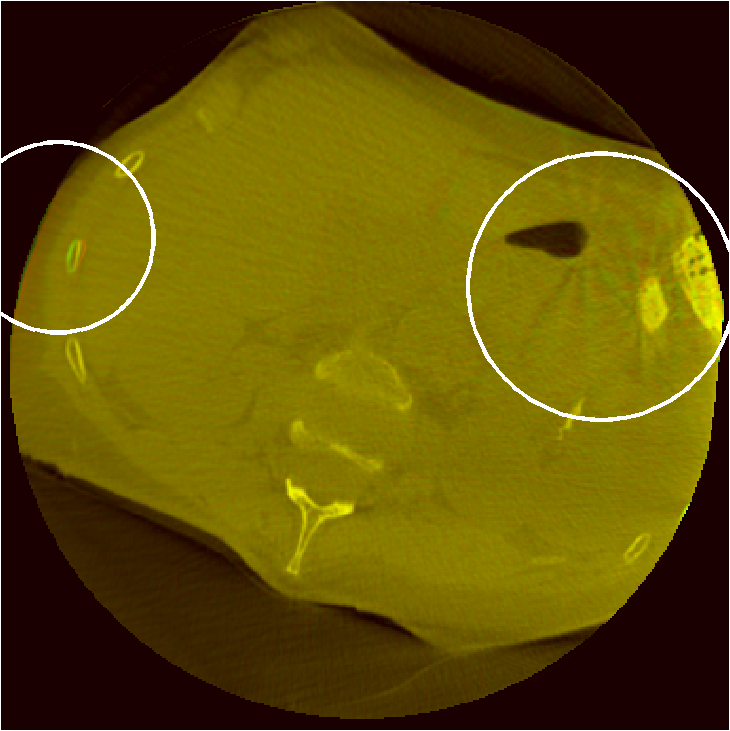
\includegraphics[width=\textwidth]{registeredSlice.png} 
\caption{After Registration} \label{regSlice} 
\end{subfigure} 
\caption{Baseline (green channel) and Comparison (red channel) Image superimposed in one image before and after registration}
\label{beforeAndAfterReg} 

\end{figure}

\subsection{Needle Detection}

The HU values for the needle and thermocouple are significantly higher than the values for normal tissue. Thus after thresholding the values in the CBCT scan high enough, the points remaining are the ones in the needle and thermocouple. Doing connected component analysis with \textbf{\href{http://www.mathworks.com/help/images/ref/bwconncomp.html}{bwconncomp}} \cite{bwconncomp} in Matlab let us find the clusters which contain the needles and thermocouples. For each component, \textbf{\href{http://www.mathworks.com/help/stats/pca.html}{pca}} \cite{pca} in Matlab was done to find the needle vector and endpoints. Figure \ref{needleDetection} shows the result after performing this procedure for one of our patients.

\begin{figure} 
\centering 
\begin{subfigure}[t]{0.45\textwidth} 
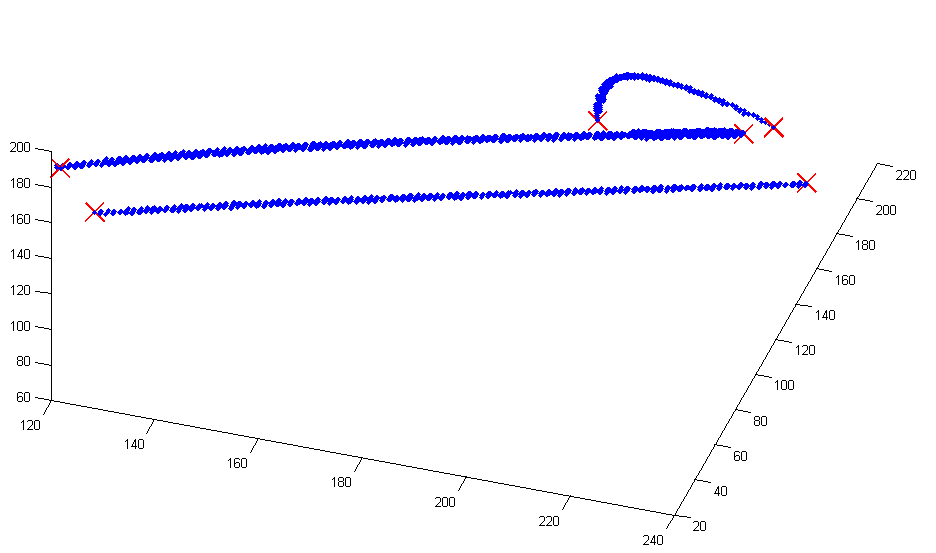
\includegraphics[width=\textwidth]{needleDetection3D_1.png}
\end{subfigure} 
\begin{subfigure}[t]{0.45\textwidth} 
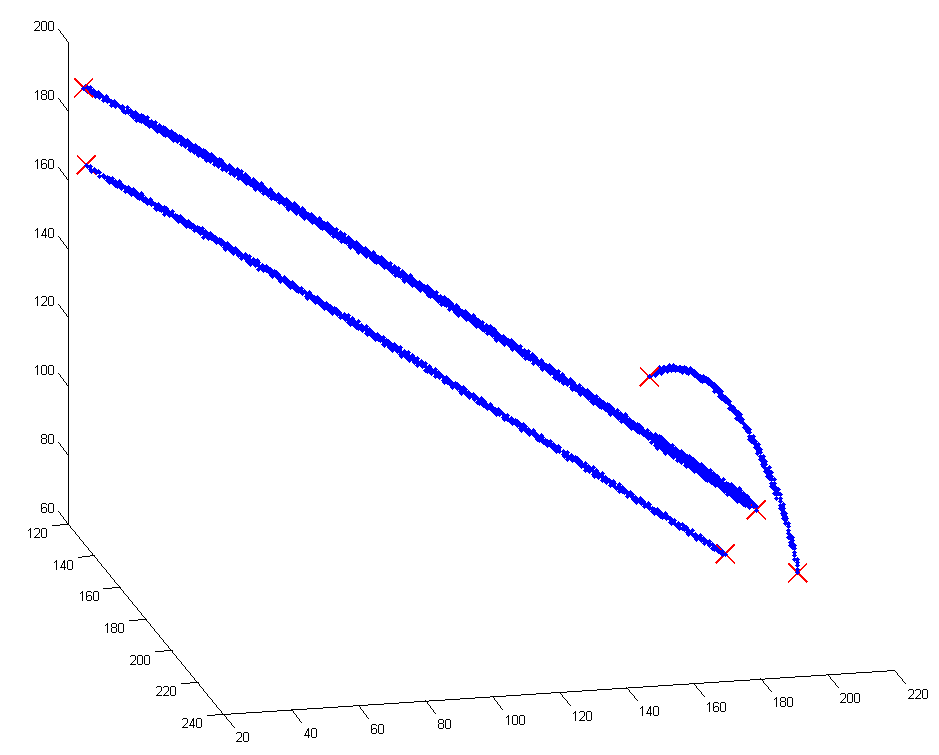
\includegraphics[width=\textwidth]{needleDetection3D_2.png} 
\end{subfigure} 
\caption{Needles and Thermocouple (blue) and their endpoints (red) detected using PCA}
\label{needleDetection} 
\end{figure}

\subsection{Change Detection}

These images have a low signal to noise ratio as well as beam hardening artifacts. We thus decided to use a window around each pixel in order to have a more robust change value. Initially we calculated the mean difference between the baseline image window and the comparison image window and used that as the value of the pixel in the result image. This is equivalent to performing a convolution on both images with an averaging filter and then taking the difference between the filtered images. The result images were used to provide an estimate of how the thermal map will appear. They are still too noisy to be used for the thermal map though. 

In order to find a better result image, for each pixel, we calculated the minimum RMSE between the baseline and comparison windows assuming that there is a spatial offset between them. 

Here is the second method procedure:
For each pixel $(i,j)$ in the result image:
\begin{enumerate}
\item Let $w$ be half-width of the window around the pixel. 
\item Let $n=2w+1$. This means the window is size $n$ by $n$. 
\item Let $U$ be window around $(i,j)$ in baseline image
\item Let $U'$ be $U$ repeated in the following way:
\[
\forall(k,l,i \in Z)\, \, \, U'_{k+i \cdot n,l+i \cdot n} = U_{k,l}
\]
\item Let $V$ be window around $(i,j)$ in the comparison image
\item Calculate the following:
\[
\min_{r,c} \sum_{l=0}^{n-1} \sum_{k=0}^{n-1} {(U'_{k+r,l+c}-V_{k,l})^2}
\]

\end{enumerate}

\begin{figure} 
\centering 
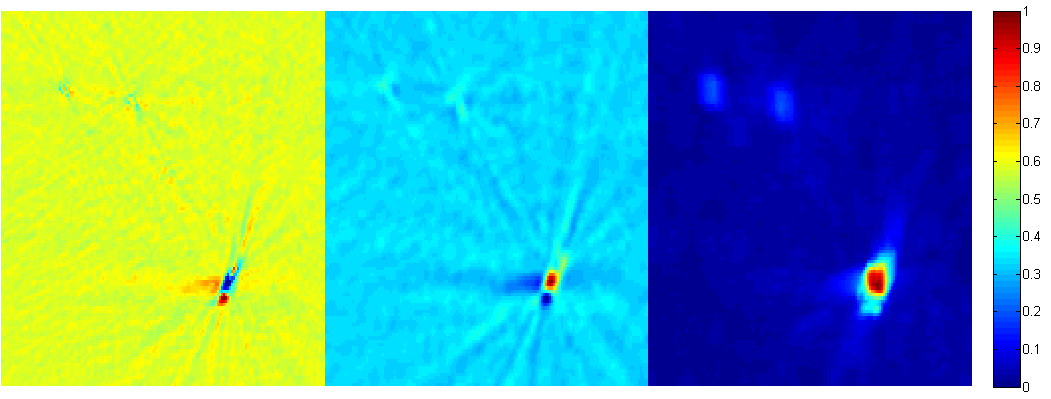
\includegraphics[width=\textwidth]{changeDetectionPanel2.png} 
\caption{Results of different change metrics in the ROI. Raw subtraction (left), Filtered Difference (center), and Sliding Window RMSE (right)} 
\end{figure}

\subsection{Regression}

After generating the sliding window image, we find the coordinates where the measured temperature zones are located. We correlate the sliding window values with the measured temperature at those zones using linear regression. We then take the regression equation found and compute its output across the sliding window image. This gives us the thermal map.  

We then took the sliding window RMSE value and calibrated it using the measured temperature change at the needle through a regression model. We used the model to calculate a thermal map in the ROI. This thermal map was used to obtain an approximate mean temperature around the needles and thermocouples.

\begin{figure} 
\centering 
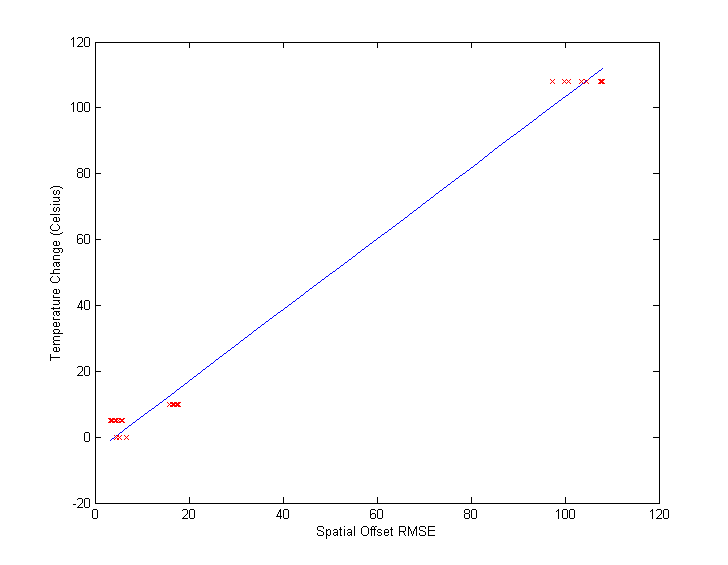
\includegraphics[width=4in]{slidingDiffRegression.png} 
\caption{Regression Curve Calculated} 
\end{figure}

\begin{figure} 
\centering 
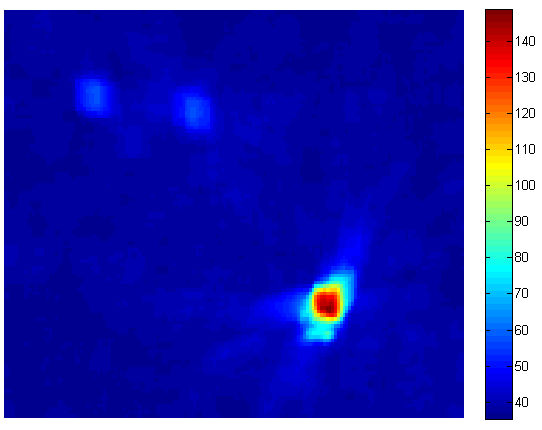
\includegraphics[width=4in]{slidingDiffThermalMap.png} 
\caption{Thermal Map generated from Regression curve} 
\end{figure}


\section{Results}

We used a data set of CBCT scans taken during 13 ablation procedures performed between September 2013 and June 2015. For each ablation procedure, there were between 1 and 4 ablations done. With each ablation, a baseline scan was taken followed by 1-4 comparison scans at different time points. Each of these time points had the ablation needle at different temperatures. We generated a thermal map at each of these time points in order to estimate the amount of tissue affected. 

\subsection{Finding Error Rates}

We decided to take the thermal maps generated from regression and see the average temperature in the zones that we were testing. We then did an RMSE of those temperatures with the measured temperatures. We dividied this RMSE by the temperature range in order to obtain an error rate. Here are the results:

**INSERT RESULT TABLE**

\subsection{Approximating Ablation Zone Area}

For the ablation zones, we made a graph of radius of region versus average temperature in that region in the thermal map. This graph can one day be used to approximate the radius of an ablation zone. Here it is for the various patients in our study. 

\begin{figure} 
\centering 
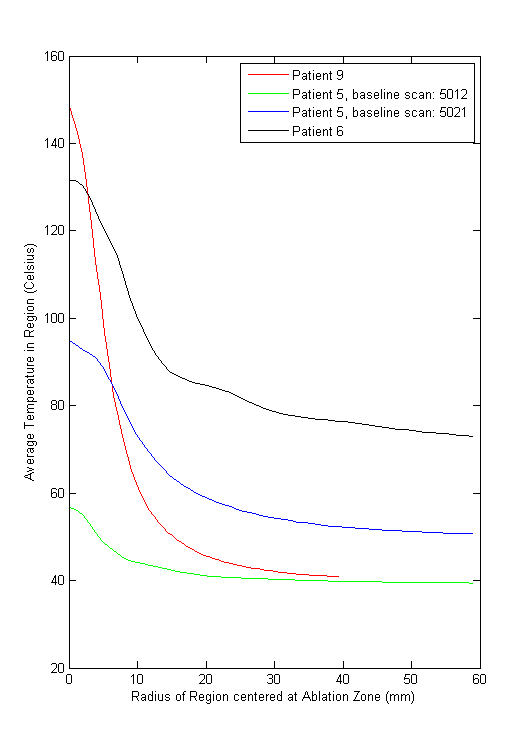
\includegraphics[width=3in]{meanTempVsRadiusFull.png} 
\caption{Shows the graph of radius vs mean temperature} 
\end{figure}


\subsection{3D Visualization of Ablation Zone}

By taking the 3D Thermal Map, thresholding the values, and then using a surface generation algorithm using \href{www.itksnap.org}{ITK-SNAP} \cite{Yushkevich06}, we were able to create a 3D diagram of the ablation zone. We overlayed the 3D diagram of the needle and we were able to obtain a convincing visual. The overlay was done in \href{http://www.slicer.org/}{3D Slicer} \cite{Fedorov12}. 

\begin{figure} 
\centering 
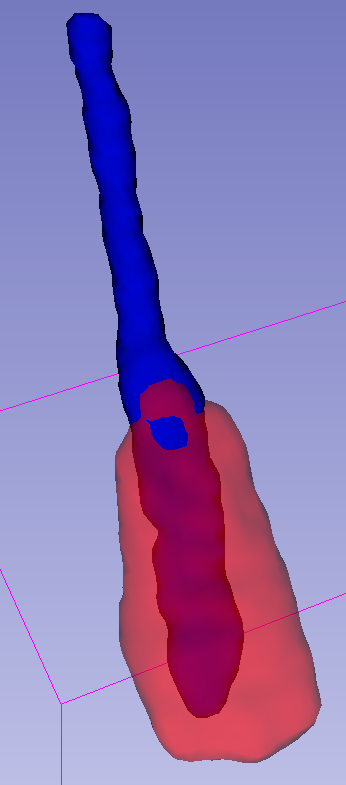
\includegraphics[width=3in]{NeedleAndAblationZone.png} 
\caption{Shows a 3D Visualization of the Needle and Ablation Zone} 
\end{figure}

\section{Conclusions and Future Work}

As can be observed, for some of the patients, our temperatures after regression were quite accurate while for others, the error was higher. The higher error was the result of a high residual value in the linear regression. This was likely caused by image noise, registration error, or user error when selecting the ROI. 

For the patients where the error was low, the methods we employed have the potential to provide useful thermal maps during ablation procedures. These thermal maps can then be used to approximate the size of the ablation zone. Additionally, there is the potential to generate a 3D visual representation of the ablation zone. 

The next step is to automate ROI selection using the needle properties. Additionally, we hope to use a data set where multiple imaging modalities were employed. That way we can test our thermal map against one generated by a modality that is known to generate accurate thermal maps. 

\subsection{Metal Artifact Deletion}

In addition to filtering, a common method to clean up these images before analysis is through Metal Deletion \cite{Boas11}. It is an active area of research.



\bibliography{report}   %>>>> bibliography data in report.bib
\bibliographystyle{spiebib}   %>>>> makes bibtex use spiebib.bst

\end{document} 
